\pdfminorversion=7
\documentclass[11pt,letterpaper]{article}
\usepackage[margin=0.85in]{geometry}
\usepackage[T1]{fontenc}
\usepackage{lmodern}
\usepackage[utf8]{inputenc}
\usepackage{graphicx}
\usepackage{xcolor}
\usepackage{enumitem}
\usepackage[
  colorlinks=true,
  linkcolor=blue!55!black,
  urlcolor=blue!55!black,
  pdftitle={Graphical Abstract and Research Highlights},
  pdfauthor={Umar Iqbal}
]{hyperref}

\definecolor{accent}{RGB}{24,74,124}
\definecolor{muted}{RGB}{85,92,102}

\begin{document}
\thispagestyle{empty}

\noindent{\Large\bfseries\color{accent} Graphical Abstract and Research Highlights (Elsevier submission material)}\par
\vspace{4pt}
\noindent\rule{\textwidth}{0.8pt}
\par\vspace{12pt}

\noindent{\large\bfseries Graphical Abstract}\par
\vspace{6pt}
\begin{center}
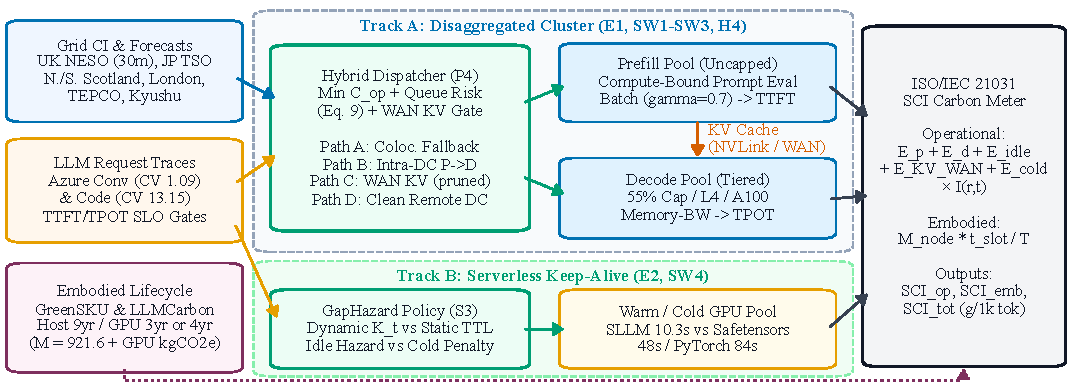
\includegraphics[width=\textwidth]{../figures/fig1_architecture.pdf}
\end{center}
\vspace{4pt}
\noindent{\small\textbf{Graphical Abstract Summary:} Dual-track ISO/IEC 21031:2024 control architecture combining four-path phase-disaggregated cluster routing (Paths A--D with WAN KV latency and carbon gating), hazard-driven serverless GPU keep-alive control, and lifecycle host plus GPU embodied carbon amortization across heterogeneous grids.}

\par\vspace{16pt}
\noindent{\large\bfseries Research Highlights ($\le 85$ characters each, verbatim from Elsevier submission)}\par
\vspace{6pt}
\begin{itemize}[leftmargin=1.5em, itemsep=5pt]
    \item PRISMA-2020 review of 65 works isolates exact multi-axis P/D carbon-routing gaps.
    \item Hybrid routing cuts operational SCI up to 60.8\% within 1\% SLO violations.
    \item WAN KV gating cuts code tail SLO violations by 85.2\%--86.0\% via Path D fallback.
    \item Hazard keep-alive trades 8.0\% dirty-grid carbon savings against clean SLO relief.
    \item Clean overprovisioning hurts at 1x (+32.7\%) but cuts SCI (-30.6\%) above 1.7x.
\end{itemize}

\vfill
\noindent\rule{\textwidth}{0.5pt}
\par\vspace{6pt}
\noindent{\footnotesize\color{muted} Author: Umar Iqbal (IILM University) \\ Code \& Reproducibility Package: \url{https://github.com/UmarIqbal000/carbon-aware-llm-scheduling}}

\end{document}
